%%%%%%%%%%%%%%%%%%%% book.tex %%%%%%%%%%%%%%%%%%%%%%%%%%%%%
%
% sample root file for the chapters of your "monograph"
%
% Use this file as a template for your own input.
%
%%%%%%%%%%%%%%%% Springer-Verlag %%%%%%%%%%%%%%%%%%%%%%%%%%


% RECOMMENDED %%%%%%%%%%%%%%%%%%%%%%%%%%%%%%%%%%%%%%%%%%%%%%%%%%%
\documentclass[envcountsame,envcountchap]{svmono}

% choose options for [] as required from the list
% in the Reference Guide, Sect. 2.2

\usepackage{makeidx}         % allows index generation
\usepackage{graphicx}        % standard LaTeX graphics tool
                             % when including figure files
\usepackage{multicol}        % used for the two-column index
\usepackage[bottom]{footmisc}% places footnotes at page bottom
\usepackage[utf8]{inputenc}
\usepackage[T1]{fontenc}
% etc.
% see the list of further useful packages
% in the Reference Guide, Sects. 2.3, 3.1-3.3

\makeindex             % used for the subject index
                       % please use the style svind.ist with
                       % your makeindex program


%%%%%%%%%%%%%%%%%%%%%%%%%%%%%%%%%%%%%%%%%%%%%%%%%%%%%%%%%%%%%%%%%%%%%

\begin{document}

\author{João Filipe Meneses Henriques\\João Nuno Santos de Gusmão Guedes}
\title{Turn 12\\
{\small FEUP-PLOG, Turma 3MIEIC05, Grupo 17}}
\subtitle{-- Monograph --}
\maketitle

\frontmatter%%%%%%%%%%%%%%%%%%%%%%%%%%%%%%%%%%%%%%%%%%%%%%%%%%%%%%

%
%%%%%%%%%%%%%%%%%%%%%%% dedic.tex %%%%%%%%%%%%%%%%%%%%%%%%%%%%%%%%%
%
% sample dedication
%
% Use this file as a template for your own input.
%
%%%%%%%%%%%%%%%%%%%%%%%% Springer-Verlag %%%%%%%%%%%%%%%%%%%%%%%%%%

\thispagestyle{empty}
\vspace*{3.5cm}
\begin{flushright}

% write your text here
{\large Your dedication goes here}

\end{flushright}




%%%%%%%%%%%%%%%%%%%%%%% pref.tex %%%%%%%%%%%%%%%%%%%%%%%%%%%%%%%%%%%%%
%
% sample preface
%
% Use this file as a template for your own input.
%
%%%%%%%%%%%%%%%%%%%%%%%% Springer-Verlag %%%%%%%%%%%%%%%%%%%%%%%%%%

\preface

%% Please write your preface here
Here come the golden words


%% Please "sign" your preface
\vspace{1cm}
\begin{flushright}\noindent
place(s),\hfill {\it First name  Surname}\\
month year\hfill {\it First name  Surname}\\
\end{flushright}




\tableofcontents


\mainmatter%%%%%%%%%%%%%%%%%%%%%%%%%%%%%%%%%%%%%%%%%%%%%%%%%%%%%%%

%%%%%%%%%%%%%%%%%%%%% chapter.tex %%%%%%%%%%%%%%%%%%%%%%%%%%%%%%%%%
%
% sample chapter
%
% Use this file as a template for your own input.
%
%%%%%%%%%%%%%%%%%%%%%%%% Springer-Verlag %%%%%%%%%%%%%%%%%%%%%%%%%%

\chapter{Resumo}
\label{abstract} % Always give a unique label
% use \chaptermark{}
% to alter or adjust the chapter heading in the running head

Este artigo foi elaborado no contexto do curso de Programação em Lógica, e incide sobre a programação em lógica com restrições. 
A programação em lógica com restrições permite restringir problemas por domínio de soluções e por condições que devem ser cumpridas. 

Com o objectivo de avaliar a viabilidade da programação com restrições para resolver problemas de lógica de complexidade relevante, foram desenvolvidos algoritmos de resolução e de geração de novas soluções para dimensões variáveis do jogo Turn 12.
Para o efeito fez-se recurso à biblioteca de restrições para o cojunto dos domínios finitos clp(FD) do SICStus Prolog.

O método utilizado compreende a rotação dos dígitos de cada face, sendo o domínio o conjunto de rotações possíveis. A combinação das faces é feita iterativamente e não simultâneamente, por forma a optimizar os recursos.

Obtiveram-se resultados em tempo útil para solucionar o problema original e para um número de digitos não superior a 60, o que permitiu concluir que a metodologia utilizada é adequada para a resolução de problemas do género.

%%%%%%%%%%%%%%%%%%%%% introduction.tex %%%%%%%%%%%%%%%%%%%%%%%%%%%%%%%%%
%
% Introduction chapter
%
%%%%%%%%%%%%%%%%%%%%%%%% Springer-Verlag %%%%%%%%%%%%%%%%%%%%%%%%%%

\chapter{Introducão}
\label{introduction} % Always give a unique label
% use \chaptermark{}
% to alter or adjust the chapter heading in the running head

Programação em lógica com restrições é uma junção de dois paradigmas: solução de restrições e programação em lógica. Esta combinação permite uma concepção mais expressiva e flexível — e em alguns casos mais eficiente - de problemas lógicos.

\section{Motivação}
\label{sec:1}
% Always give a unique label
% and use \ref{<label>} for cross-references
% and \cite{<label>} for bibliographic references
% use \sectionmark{}
% to alter or adjust the section heading in the running head
A motivação deste trabalho incidiu na compreensão de um paradigma de programação que já nos é familiar, envolvendo uma nova componente de restrições; resolver problemas lógicos com restrições de uma forma geral, tendo a possibilidade de os refinar e otimizar para uma solução particular.

\section{Objectivos}
\label{sec:2}
Resolver a versão original do jogo Turn12 recorrendo a restrições; gerar cubos com um número de dígitos variável, e avaliar se estes têm solução ou não segundo as restrições definidas.

\section{Descrição do problema}
\label{sec:3}
O problema centra-se num cubo em que cada face contém dígitos numerados de 3 a 9, aleatoriamente. Na junção das arestas de cada face, a soma dos dois dígitos que se encontram deverá ser igual a 12.

A solução original (Fig. 2.1) com 24 dígitos por face é única.

A resolução que apresentamos contempla dígitos ilimitados, e uma vez que não existe qualquer padrão associado à sequência de dígitos no problema original, estes são gerados aleatóriamente e não é garantida a unicidade de solução.

No entanto, para valores demasiado elevados (superiores a 60 por face), as limitações de computação começaram-se a sentir e encontrar uma solução em tempo útil não foi possível, por limitações de Hardware.

%Figura cubo
\begin{figure}[h!]
\begin{center}
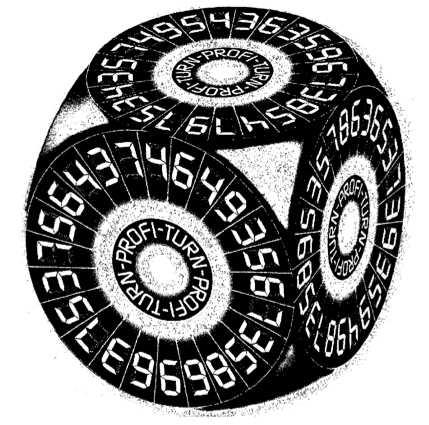
\includegraphics[scale=0.4]{turn12.png}
\caption{Problema original}
\label{fig:1}
\end{center}
\end{figure}

%


%\appendix
%\include{appendix}

\backmatter%%%%%%%%%%%%%%%%%%%%%%%%%%%%%%%%%%%%%%%%%%%%%%%%%%%%%%%

\chapter*{Solutions}
\addcontentsline{toc}{chapter}{Solutions}
\markboth{Solutions}{Solutions}

\section*{Problems of Chapter~\ref{intro}}

\begin{sol}{prob1}
The solution is revealed here.
\end{sol}


\begin{sol}{prob2}
\textbf{Problem Heading}\\
(a) The solution of first part is revealed here.\\
(b) The solution of second part is revealed here.
\end{sol}


%%%%%%%%%%%%%%%%%%%%%%%% referenc.tex %%%%%%%%%%%%%%%%%%%%%%%%%%%%%%
% sample references
% "computer science"
%
% Use this file as a template for your own input.
%
%%%%%%%%%%%%%%%%%%%%%%%% Springer-Verlag %%%%%%%%%%%%%%%%%%%%%%%%%%

%
% BibTeX users please use
% \bibliographystyle{}
% \bibliography{}
%
% Non-BibTeX users please use
\begin{thebibliography}{99.}
%
% and use \bibitem to create references.
%
% Use the following syntax and markup for your references
%
% Monographs
\bibitem{monograph} Kajan E (2002)
Information technology encyclopedia and acronyms. Springer, Berlin
Heidelberg New York

% Contributed Works
\bibitem{contribution} Broy M (2002) Software engineering -- From
auxiliary to key technologies. In: Broy M, Denert E (eds)
Software Pioneers. Springer, Berlin Heidelberg New York

% Journal
\bibitem{journal} Che M, Grellmann W, Seidler S (1997)
Appl Polym Sci 64:1079--1090

% Theses
\bibitem{thesis} Ross DW (1977) Lysosomes and storage diseases. MA
Thesis, Columbia University, New York

\end{thebibliography}

\printindex

%%%%%%%%%%%%%%%%%%%%%%%%%%%%%%%%%%%%%%%%%%%%%%%%%%%%%%%%%%%%%%%%%%%%%%

\end{document}





